%%%%%%%%%%%%%%%%%%%%%%%%%%%%%%%%%%%%%%%%%
% Journal Article
% LaTeX Template
% Version 1.4 (15/5/16)
%
% This template has been downloaded from:
% http://www.LaTeXTemplates.com
%
% Original author:
% Frits Wenneker (http://www.howtotex.com) with extensive modifications by
% Vel (vel@LaTeXTemplates.com)
%
% License:
% CC BY-NC-SA 3.0 (http://creativecommons.org/licenses/by-nc-sa/3.0/)
%
%%%%%%%%%%%%%%%%%%%%%%%%%%%%%%%%%%%%%%%%%

%----------------------------------------------------------------------------------------
%	PACKAGES AND OTHER DOCUMENT CONFIGURATIONS
%----------------------------------------------------------------------------------------

\documentclass[twoside,twocolumn]{article}

\usepackage{blindtext} % Package to generate dummy text throughout this template 

\usepackage[sc]{mathpazo} % Use the Palatino font
\usepackage[T1]{fontenc} % Use 8-bit encoding that has 256 glyphs
\linespread{1.05} % Line spacing - Palatino needs more space between lines
\usepackage{microtype} % Slightly tweak font spacing for aesthetics

\usepackage[english]{babel} % Language hyphenation and typographical rules

\usepackage[hmarginratio=1:1,top=32mm,columnsep=20pt]{geometry} % Document margins
\usepackage[hang, small,labelfont=bf,up,textfont=it,up]{caption} % Custom captions under/above floats in tables or figures
\usepackage{booktabs} % Horizontal rules in tables

\usepackage{lettrine} % The lettrine is the first enlarged letter at the beginning of the text

\usepackage{enumitem} % Customized lists
\setlist[itemize]{noitemsep} % Make itemize lists more compact

\usepackage{abstract} % Allows abstract customization
\renewcommand{\abstractnamefont}{\normalfont\bfseries} % Set the "Abstract" text to bold
\renewcommand{\abstracttextfont}{\normalfont\small\itshape} % Set the abstract itself to small italic text

\usepackage{titlesec} % Allows customization of titles
\renewcommand\thesection{\Roman{section}} % Roman numerals for the sections
\renewcommand\thesubsection{\roman{subsection}} % roman numerals for subsections
\titleformat{\section}[block]{\large\scshape\centering}{\thesection.}{1em}{} % Change the look of the section titles
\titleformat{\subsection}[block]{\large}{\thesubsection.}{1em}{} % Change the look of the section titles

\usepackage{fancyhdr} % Headers and footers
\pagestyle{fancy} % All pages have headers and footers
\fancyhead{} % Blank out the default header
\fancyfoot{} % Blank out the default footer
\fancyhead[C]{Adrien Cogny $\bullet$ Apr 2018} % Custom header text
\fancyfoot[RO,LE]{\thepage} % Custom footer text

\usepackage{titling} % Customizing the title section

\usepackage{hyperref} % For hyperlinks in the PDF

\usepackage{float}

\usepackage{graphicx} % added graphix package for images
\graphicspath{ {images/} } 


%----------------------------------------------------------------------------------------
%	TITLE SECTION
%----------------------------------------------------------------------------------------

\setlength{\droptitle}{-4\baselineskip} % Move the title up

\pretitle{\begin{center}\Huge\bfseries} % Article title formatting
\posttitle{\end{center}} % Article title closing formatting
\title{User Response Classification Challenge} % Article title
\author{%
\textsc{Adrien Cogny} \\% Your name
\normalsize Cornell Tech \\ % Your institution
\normalsize \href{mailto:ac2753@cornell.edu}{ac2753@cornell.edu} % Your email address
%\and % Uncomment if 2 authors are required, duplicate these 4 lines if more
%\textsc{Jane Smith}\thanks{Corresponding author} \\[1ex] % Second author's name
%\normalsize University of Utah \\ % Second author's institution
%\normalsize \href{mailto:jane@smith.com}{jane@smith.com} % Second author's email address
}
\date{\today} % Leave empty to omit a date
\renewcommand{\maketitlehookd}{%
\begin{abstract}
\noindent Abstract Text % Dummy abstract text - replace \blindtext with your abstract text
\end{abstract}
}

%----------------------------------------------------------------------------------------

\begin{document}

% Print the title
\maketitle

%----------------------------------------------------------------------------------------
%	ARTICLE CONTENTS
%----------------------------------------------------------------------------------------

\section{Introduction}

\lettrine[nindent=0em,lines=3]{C}hatbots are used in many applications today: customer support,
flight booking, scheduling meeting, ordering food and many more. The application of a chatbot
 explored in this dataset is for a therapy chatbot. These types of chatbot, while very effective,
 may require human intervention. Determining when a human should intervene can be quite important,
 in this case when a person requires help in dealing with a complex situation, and requires tools
 to identify these situations. 

The data set contains 80 examples of responses entered into a therapy chatbot. Each of these responses
contains an id as well as an identification. The identification is either "flagged" if the response
was flagged for human intervention or "not flagged" if not.

The task at hand was to create an AI agent to classify the user response. 
%------------------------------------------------

\section{Tools}

The following tools and modules were used to complete this task:
\begin{itemize}
\item python 3.6.5 (using conda)
\item pandas (0.22.0)
\item dy-net (for the RNN) (2.0)
\item scikit learn (for the Random Forest) (0.19.1)
\item numpy (1.14.2)
\item tqdm (for progress bars) (4.22.0)
\item csv (For reading the csv embeddings to pandas) (1.0)
\item re (regular expressions) (for cleaning the data) (2.2.1)
\end{itemize}
 

%------------------------------------------------
\section{Preparing Data}
The input data being sentences had to be cleaned up before passing into the models.

The first step was to load the csv file into a pandas dataframe and see what the data looked like.
The data was, as mentioned above, a label as well as a sequence of words (not an array implementation yet).
Due to the inherent nature of natural language processing both the label and sequence of words had to
be converted to something which the machine could understand. That is, the label had to be converted from 
"flagged" or "not flagged" to 1 or 0 respectively and the sequence had to be converted to a series of word
embeddings where each embedding represented a single word.

Natural language contains many words that are very common in sentences. These so-called stop words
 ("their", "he", "she", etc...) can make classifying a sentence very hard as, when combining word
 embeddings, they will take over the representation of the sentence simply by shear number. That is 
 why in the pre-processing of each sentence (before it is given to the model), the stop words were removed
 from the sentence. By removing the stop words, we do not loose much important information and
 are able to classify more easily.

The models were created to do the conversion from label to 1 or 0 and from sentence of words to sequence of embeddings.
The embeddings used were the GloVe 6B embeddings which come from wikipedia scapping\footnote{https://nlp.stanford.edu/projects/glove/}.


\section{Models}

\subsection{RNN}

When looking at sentence classification, one of the first thought was too look at an RNN encoder
that would encode the sentence word by word and the computing a probability of being "flagged"
or "not flagged". The label with the highest probability would then be applied to the sentence input.

\subsubsection{RNN Description}

DESCRIPTION OF RNN AND IMAGE/SKETCH OF THE MODEL CRATED

\subsubsection{Tuning Parameters}

When the model was created, the different parameters were tuned:
\begin{itemize}
  \item{Embedding Dimmension}
  \item{Hidden Dimmension Size}
  \item{Number of Epochs Run}
\end{itemize}

The results for all of these tuning experiments are shown in the results section.


\subsection{Random Forest}

After getting results for the RNN encoder and finding the best possible RNN,
it was posited (based on research into text classification) that a random
forest classifier could be more apt at this task.

\subsubsection{Random Forest Description}

RANDOM FOREST DESCRIPTION

\subsubsetion{Tuning Parameters}
When the model was created, the different parameters were tuned:

\begin{itemize}
  \item{Number of Estimators}
  \item{Sentence to Embedding Methodology} 
\end{itemize}

Whereas the number of estimators is a property of the random forest model itself,
the sentence to embedding methodology describes how a sentences (or rather sequence of words)
is transformed into a single vector wich can be input to the Random forest model.

There were two methods for embedding the sentence. One was to compute the mean of all the
word embeddings and the other to compute the sum. The mean would attempt to construct a mean
representation of the sentence using all the words in the sentence. The summation would create
a sentence which was a sum of its parts.

%------------------------------------------------

\section{Results}

\subsection{RNN}

\subsubsection{Hidden dimmension}

The hidden dimmension test was done by keeping all parameters of the RNN constant except for the 
hidden dimmension of the RNN. The following figure shows the results for the hidden dimmension
test performed. The test was performed by changing the size of the embedding dimmension from 0 to 9
dimmensions in steps of 1. The training loss, dev set true positive #, dev set true negative #,
dev set false positive # and dev set false negative # were computed for each of the models run 
and a graph was created showing the true positive rate and the false positive rate.

\begin{figure}[H]
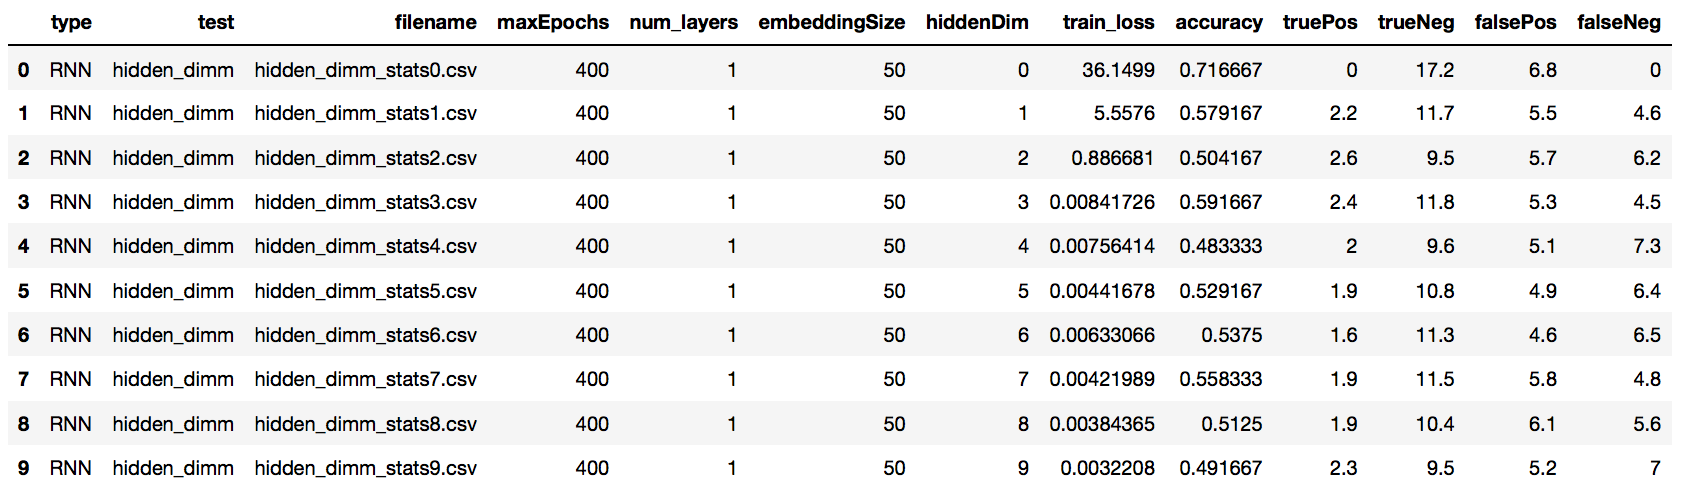
\includegraphics[width=6cm]{hidden_dimm_test_table}
\centering
\caption{Shows the table of hidden dimmension tests for the RNN}
\end{figure}

\begin{figure}[H]
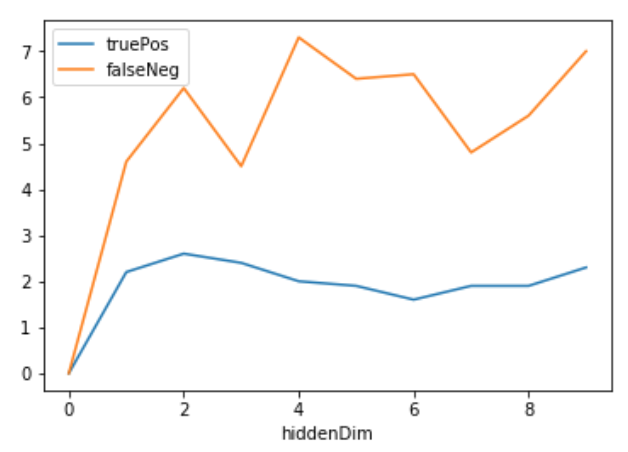
\includegraphics[width=6cm]{hidden_dimm_test_graph}
\centering
\caption{Shows the graph of true positive count vs hidden dimmension of RNN}
\end{figure}

This graph shows that the true positive count is always lower than the false negative count.
This means that there are more instances where the model will classify a sentence as "not flagged"
when in fact it should be "flagged" than there are instances where the model correctly classifies
a sentence as "flagged." While this points towards this particular model
(with the hyperparameters described below) not being good, the true positive rate and accuracies are
derived (and much more important) metrics to look at.

While this graphs shows the true positive count as well as the false negative counts,
a more interesting metric which can be derived fromt he true positive count and
the false negative count is the true positive rate (tpr) which shows how much 
of the truth the model captures.

The following figure shows the tpr for the RNN model for different hidden dimmensions.

\begin{figure}[H]
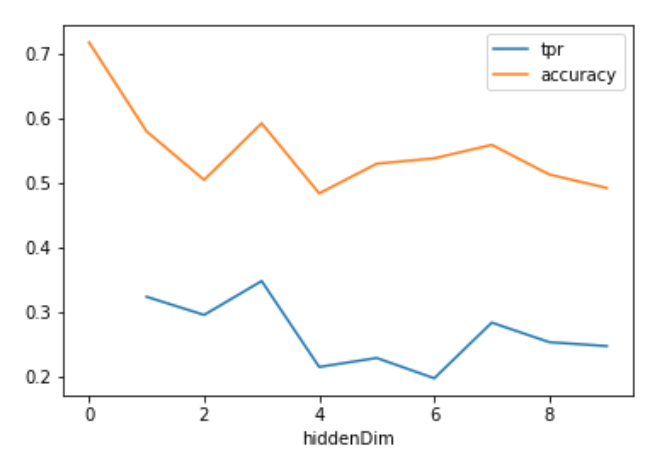
\includegraphics[width=6cm]{hidden_dimm_test_tpr-graph}
\centering
\caption{Shows the graph of true positive rate vs hidden dimmension of RNN}
\end{figure}

From this figure, we can clearly see that the tpr is greatest when the hidden dimmension is 3,
 with the other parameters set to: number of epochs ran = 400, number of layers = 1 and embedding 
 size = 50. This model received an accuracy of 0.591667 and a true positive rate of 0.347826.

While the graph of accuracies shows that when the hidden dimension is of size 0, the accuracy jumps
to ~0.7, this model would not be considered to be a good model as the true positive rate is non existant
because we are not classifying any results as being "flagged", which defeats the whole purpose of the model.

Thus, the hidden dimmension will be set to 3 for the other models.

\subsubsection{GloVe embedding size}

When the hidden dimmension was found, the next hyper-parameter which could be tuned was the size
of the GloVe embeddings used to conver the sentences into something the models could understand.

This next figure shows the true positive counts and false negative counts for each embedding dimmension
available (50, 100, 200 and 300).

\begin{figure}[H]
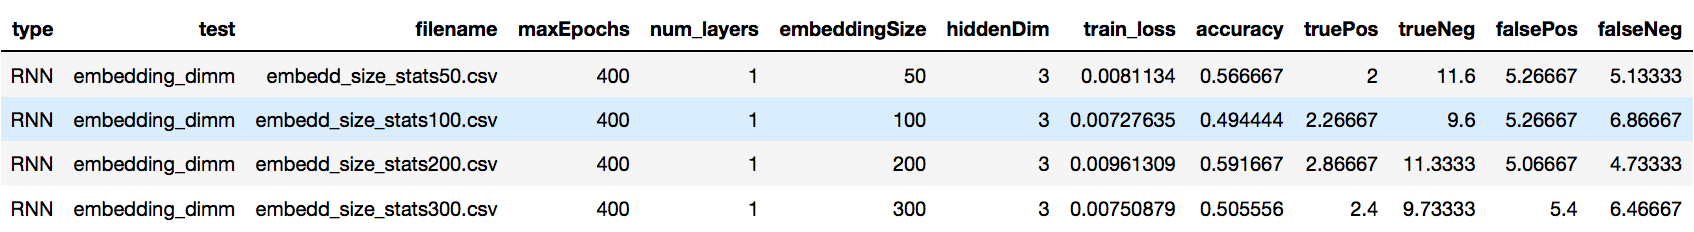
\includegraphics[width=6cm]{rnn_embeddSize_test_table}
\centering
\caption{Shows the table of embedding dimmension tests for the RNN}
\end{figure}

\begin{figure}[H]
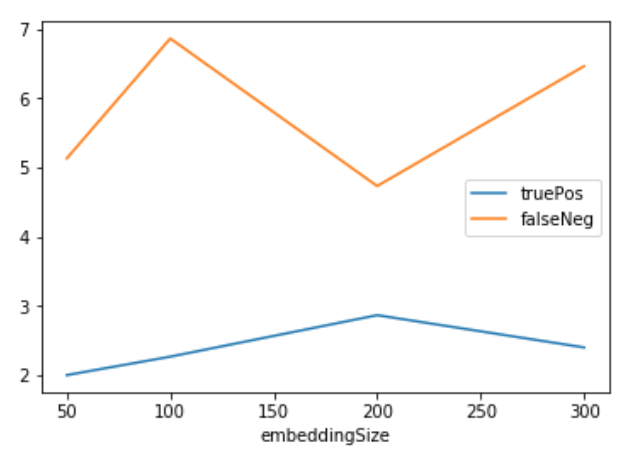
\includegraphics[width=6cm]{rnn_embeddSize_test_graph}
\centering
\caption{Shows the graph of true positive count and false negative count vs embedding dimmensions of RNN}
\end{figure}

The table and graph show that the true positive count is always smaller than the false negative count.
However a dip can be seen in the false negative count at an embedding size of 200. This dip in
false negatives is coupled by a rise in the true positive. This indicates that the embedding size of 200
yields the best results. \footnote{Note that the increase in the true positive count and decrease in false
negative counts graphed are not the same magnitude as the samples were drawn randomly from the training
set and thus may not always contain the same number of positive and negative examples.}

Confirmation of this is seen in the figures below as both the true positive rate and accuracy
are highest at an embedding size of 200.

\begin{figure}[H]
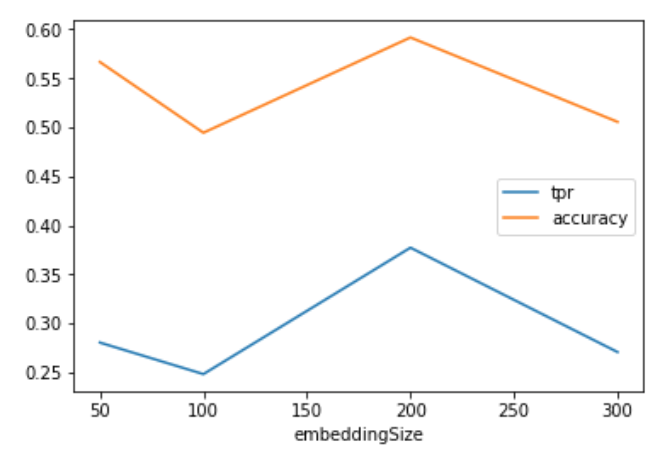
\includegraphics[width=6cm]{rnn_embeddSize_test_tpr-graph}
\caption{Shows the graph of true positive rate vs embedding dimmensions of RNN}
\centering
\end{figure}


However uppon further investigation, it seems that this may have been a random occurance due to the
randomization of the data. After running this test several times, the graph did not show any significant
improvement. For example, the following two figures was another run which illustrates that, depending
on the random set of data, the best embeddings  chnage

\begin{figure}[H]
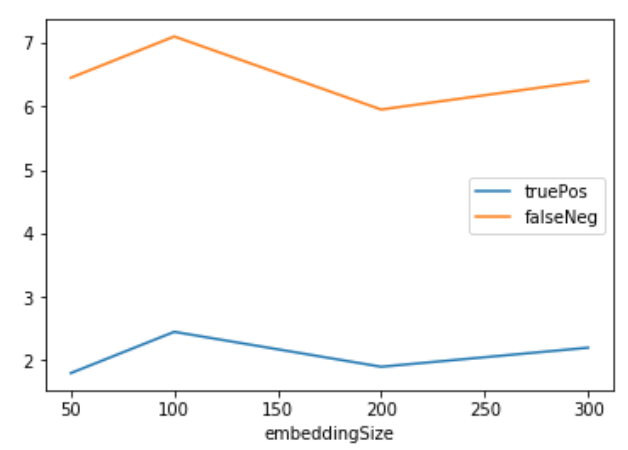
\includegraphics[width=6cm]{rnn_embeddSize_test_graph1}
\centering
\end{figure}


\begin{figure}[H]
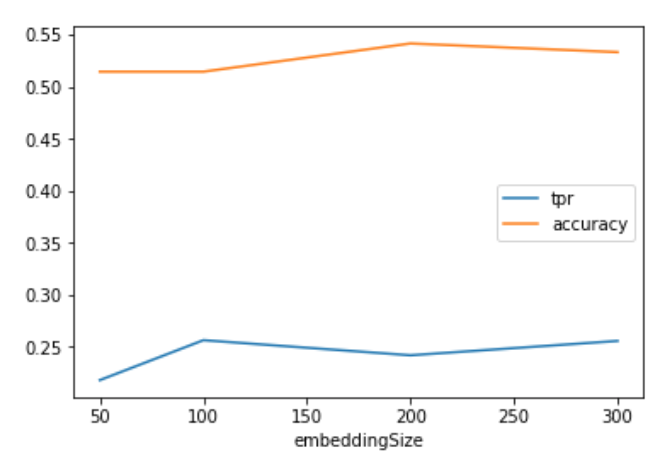
\includegraphics[width=6cm]{rnn_embeddSize_test_tpr-graph1}
\centering
\end{figure}

Therefore, for computation purposes, the embedding size was set to 100. This was thought to be
a good compromise between a larger embedding which may provide more information and the speed 
of loading the embeddings.

\subsubsection{Number Layers}

The final hyperparameter to be tuned was the number of layers that the rnn contained. Before this
test, the RNNs trained had a single layer. This test was performed twice in order to make sure there
 was consistency among even more random samples. The number of layers of the rnn were varied
 from 1 to 25 in increments of 1 for both tests.

 The first test's graph shows the number of layers vs true positive count and false negative count is shown below:

\begin{figure}[H]
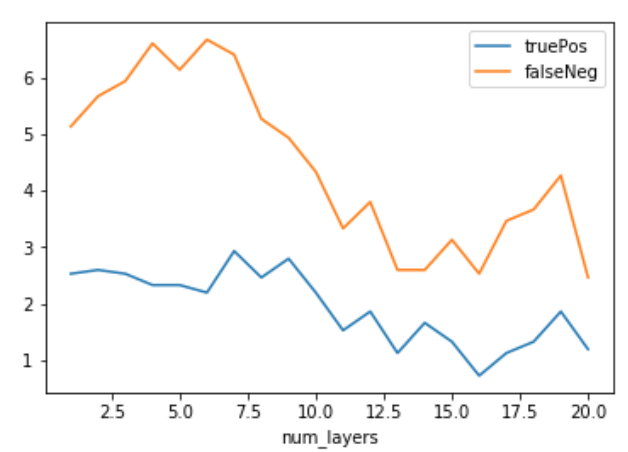
\includegraphics[width=6cm]{rnn_numberLayers_test1}
\caption{Shows the graph of true positive rate vs number of layers of RNN for the first trial}
\centering
\end{figure}

\begin{figure}[H]
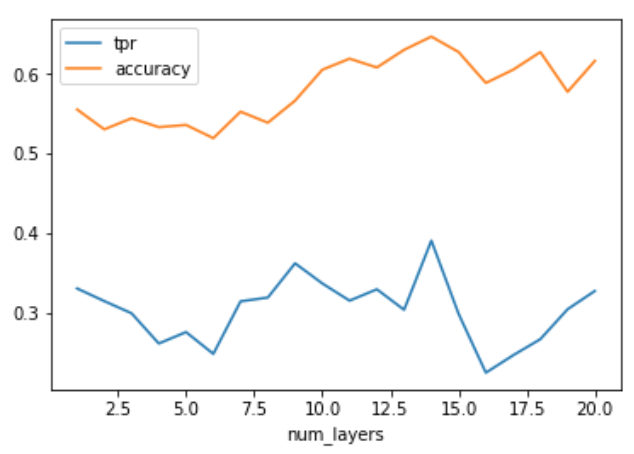
\includegraphics[width=6cm]{rnn_numberLayers_test1-tpr}
\caption{Shows the graph of true positive rate vs number of layers of RNN for the first trial}
\centering
\end{figure}

The second test's graph shows the same statistics as the previous one but for the second trial

\begin{figure}[H]
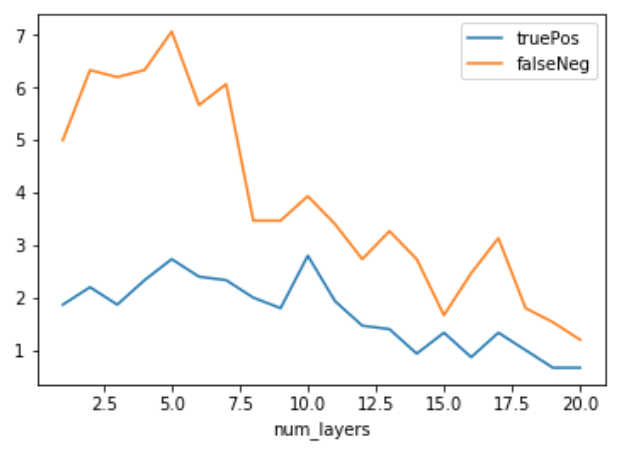
\includegraphics[width=6cm]{rnn_numberLayers_test2}
\caption{Shows the graph of true positive rate vs number of layers of RNN for the second trial}
\centering
\end{figure}
  
\begin{figure}[H]
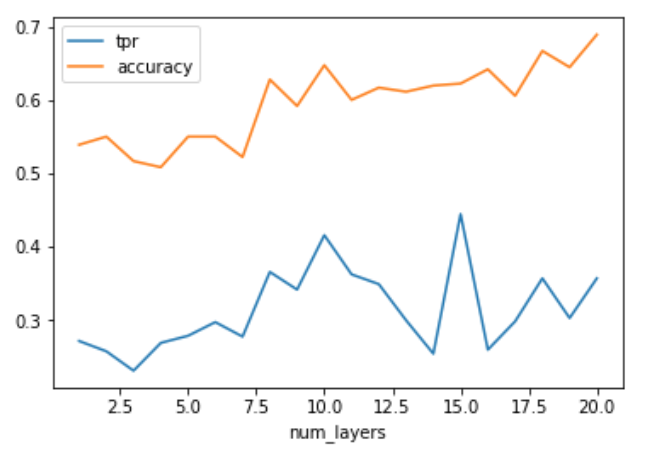
\includegraphics[width=6cm]{rnn_numberLayers_test2-tpr}
\caption{Shows the graph of true positive rate vs number of layers of RNN for the second trial}
\centering
\end{figure}

Both of these tests show that as the number of layers in the rnn increases the number of false
negatives also increases. While the exact number of layers cannot be tuned very accuractely
due to the fairly small dataset, it can be said that around 15 layers seems to be a fairly good point. 
That is because both the accuracy and the true positive rates are 


\subsubsection{RNN Final Model}





\subsection{Random Forest}

As mentioned above, when the best rnn model was tuned it yielded an accuracy of 


\subsubsection{Summation Methodology}

\begin{figure}[H]
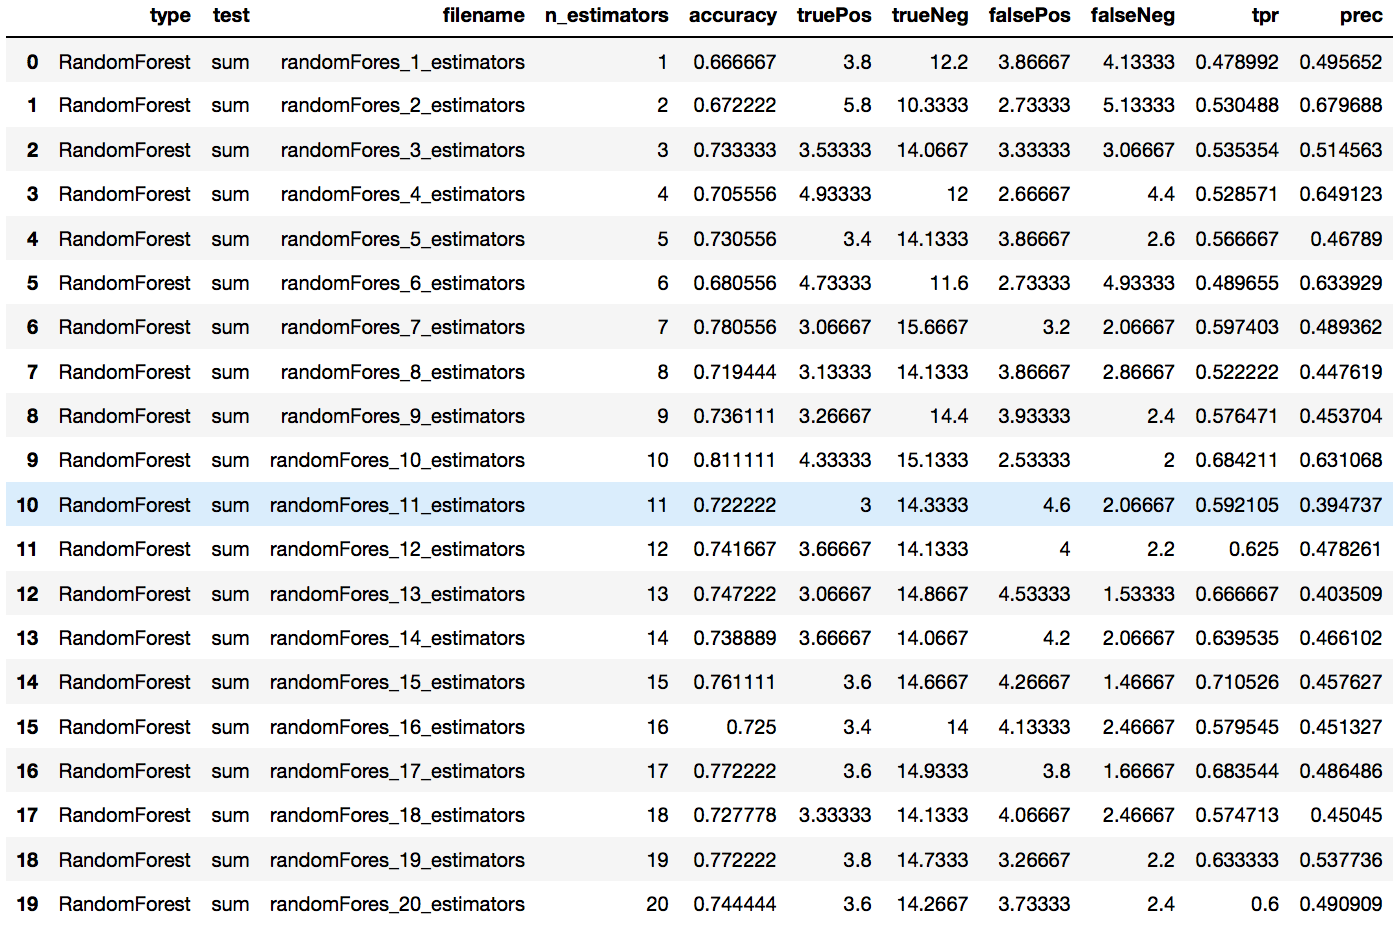
\includegraphics[width=6cm]{randForest_estimators_summed_table}
\centering
\caption{Shows the table for the experiments where the number of estimators used
in the random forest classifier were used. This is for the summation methodology.}
\end{figure}

\begin{figure}[H]
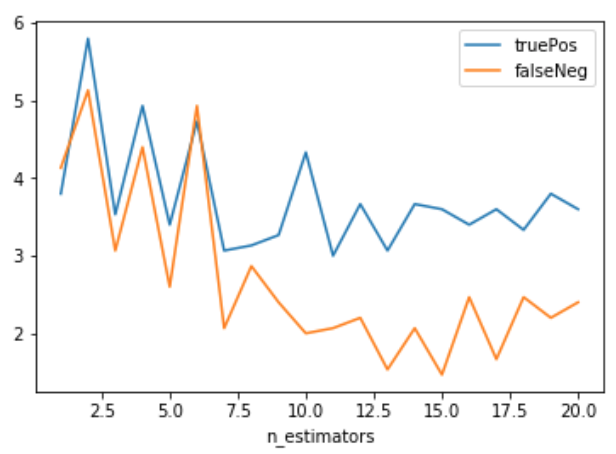
\includegraphics[width=6cm]{randForest_estimators_summed_graph}
\centering
\caption{Shows the graph for the experiments where the number of estimators used
in the random forest classifier were used. This is for the summation methodology.}
\end{figure}

\begin{figure}[H]
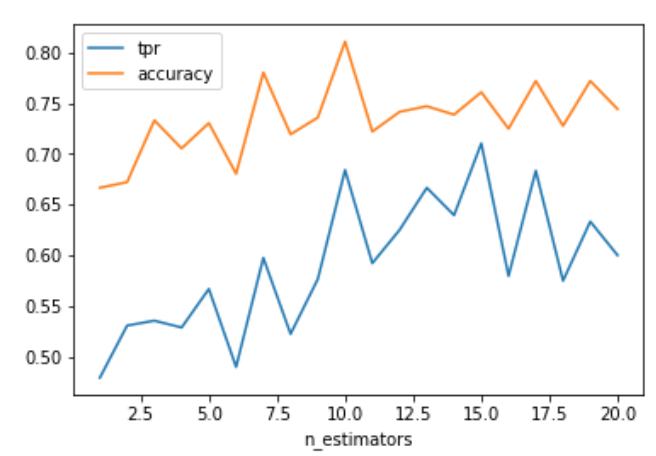
\includegraphics[width=6cm]{randForest_estimators_summed_graph-tpr}
\centering
\caption{Shows the graph of true positive rate and accuracy vs number of estimators of random forest 
with summed embeddings as representation for the sentence}
\end{figure}


\subsubsection{Mean Methodology}

\begin{figure}[H]
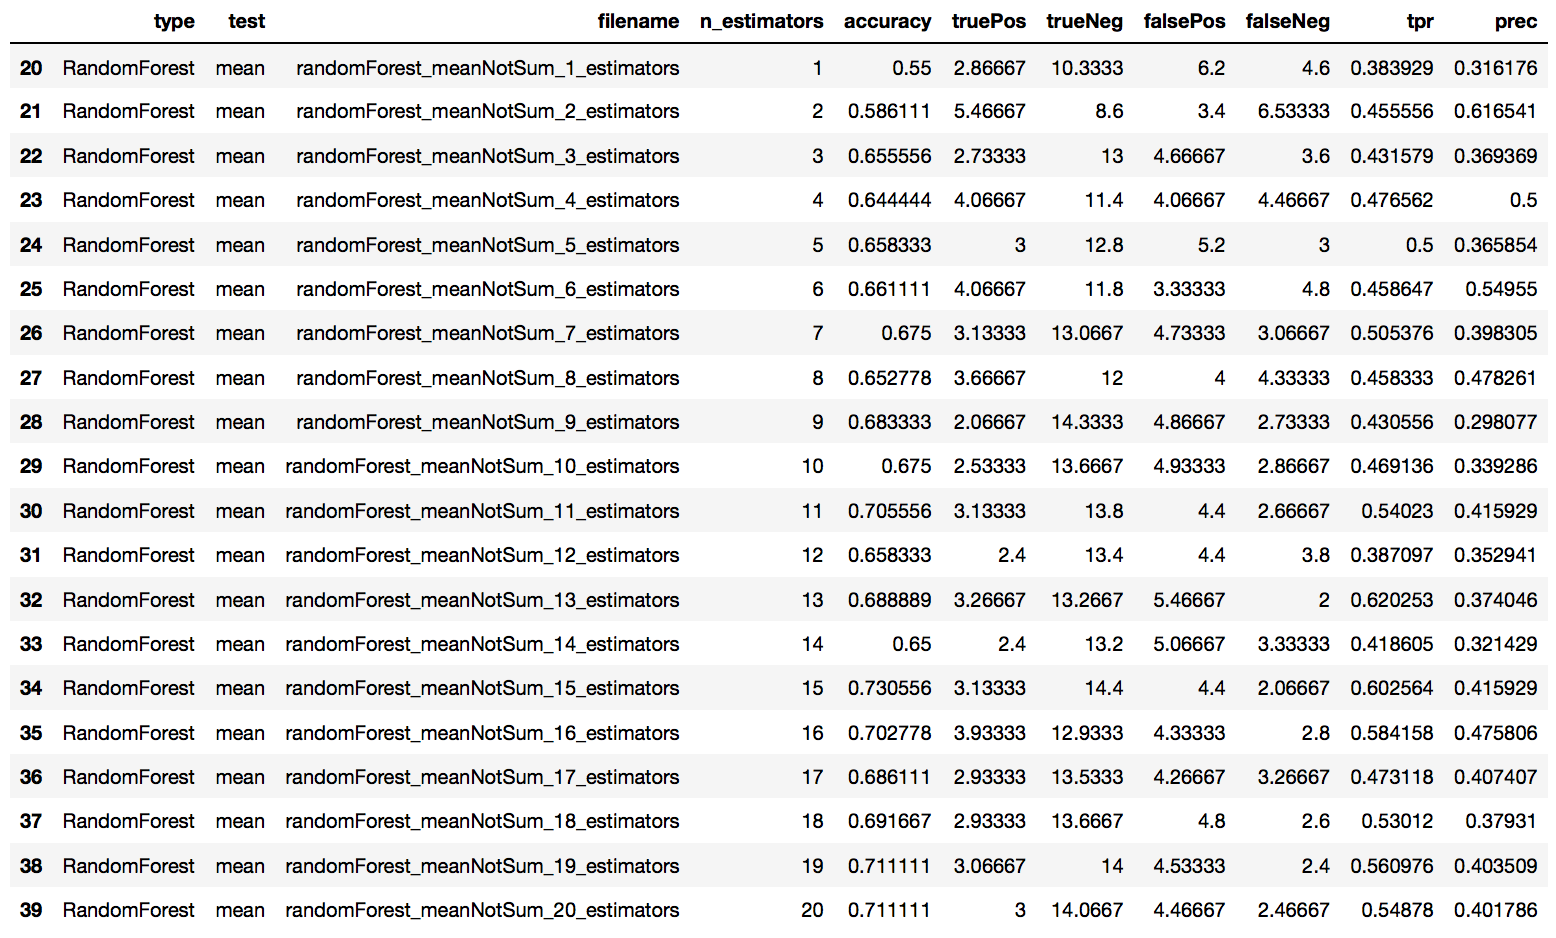
\includegraphics[width=6cm]{randForest_estimators_meaned_table}
\centering
\caption{Shows the table for the experiments where the number of estimators used
in the random forest classifier were used. This is for the mean methodology.}
\end{figure}

\begin{figure}[H]
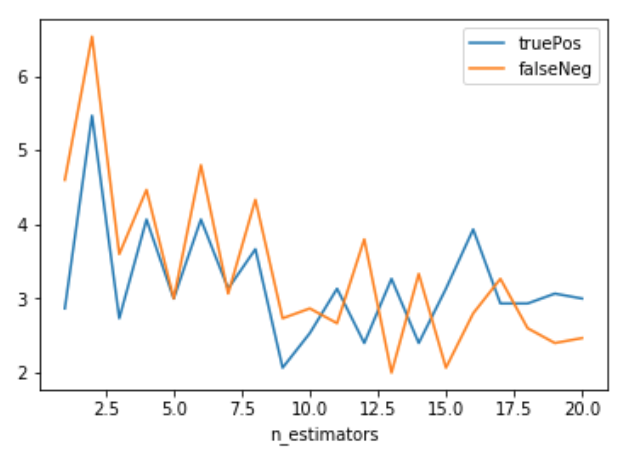
\includegraphics[width=6cm]{randForest_estimators_meaned_graph}
\centering
\caption{Shows the graph for the experiments where the number of estimators used
in the random forest classifier were used. This is for the summation methodology.}
\end{figure}

\begin{figure}[H]
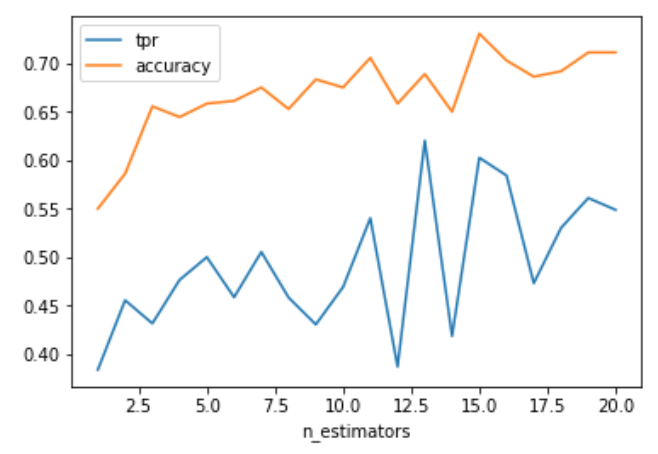
\includegraphics[width=6cm]{randForest_estimators_meaned_graph-tpr}
\centering
\caption{Shows the graph of true positive rate and accuracy vs number of estimators of random forest 
with summed embeddings as representation for the sentence}
\end{figure}


\subsubsection{Mean vs Summation Methodology}

From the figures above, it can be seen that, for all numbers of estimators used in the
random forest mode the summation accuracy and true positive rates are higher than the mean
methodology. This makes sense as the summation method attempts to feed the model the summation
of the words rather than the average representation.

\subsubsection{Random Forest Final Model}

The final model for the random forest had the following paramters:

\subsection{Final Model}

\subsection{Using the Model & Explanation of Code}


%----------------------------------------------------------------------------------------
%	REFERENCE LIST
%----------------------------------------------------------------------------------------

\begin{thebibliography}{99} % Bibliography - this is intentionally simple in this template

\bibitem[Figueredo and Wolf, 2009]{Figueredo:2009dg}
Figueredo, A.~J. and Wolf, P. S.~A. (2009).
\newblock Assortative pairing and life history strategy - a cross-cultural
  study.
\newblock {\em Human Nature}, 20:317--330.
 
\end{thebibliography}

%----------------------------------------------------------------------------------------

\end{document}
